\begin{frame}{Goals}
  \begin{itemize}
    \item Extend support for diverse microcontroller architectures.
    \item Target ISAs include ARM Cortex-M and AVR.
    \item Enable modeling of custom peripherals and I/O devices.
    \item Incorporate interrupt-driven architecture support.
    \item Facilitate real-time performance analysis and monitoring.
    \item Provide tools for debugging and execution trace visualization.
  \end{itemize}
\end{frame}

\begin{frame}{System Overview}
  \centering
  \begin{figure}
    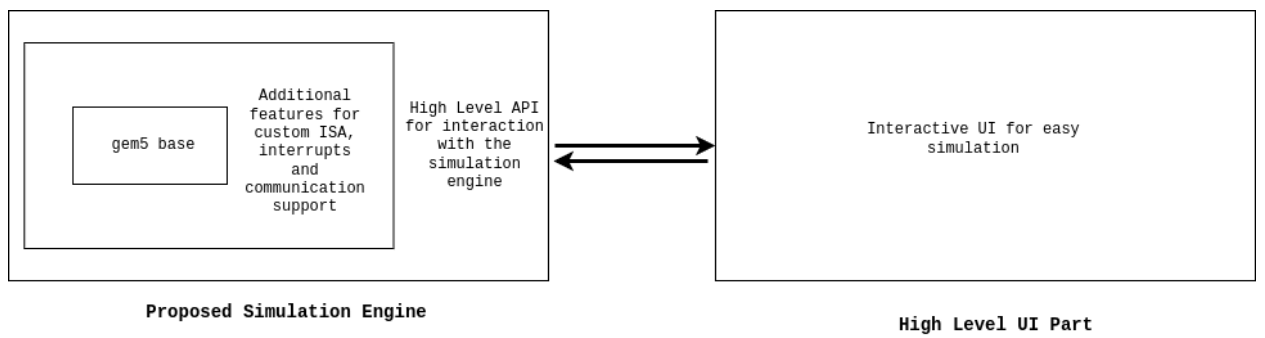
\includegraphics[width=1.0\textwidth]{images/proposed_system.png}
  \end{figure}
  \textbf{Figure 2: }Proposed System Architecture
\end{frame}

\begin{frame}{Why It Matters}
  \begin{itemize}
    \item \textbf{Microcontrollers power the embedded world} — from smart homes to medical devices.
    \item Existing GEM5 support focuses mainly on general-purpose computing architectures.
    \item Extending GEM5 enables researchers to:
    \begin{itemize}
      \item Model real-world embedded and IoT systems.
      \item Explore architectural trade-offs in low-power environments.
      \item Test RTOS behavior and peripheral interactions in a controlled simulation.
    \end{itemize}
    \item Opens doors for hardware-software co-design in constrained systems.
    \item Facilitates early-stage development and validation of next-gen embedded solutions.
  \end{itemize}
\end{frame}

\begin{frame}{Why It Matters}
  \begin{itemize}
    \item \textbf{Existing Simulators:}
    \begin{itemize}
      \item \textit{AVR Simulator, SimAVR, Proteus:} Limited scope, vendor-specific.
      \item \textit{QEMU:} General-purpose, lacks fine-grained modeling for peripherals and interrupts in microcontrollers.
      \item \textit{Renode:} Powerful, but more focused on specific embedded use cases.
    \end{itemize}
    \item \textbf{Limitations:}
    \begin{itemize}
      \item Minimal hardware-software co-design flexibility.
      \item Limited extensibility for new ISAs and custom architectures.
      \item Often lack integrated performance profiling and debugging tools.
    \end{itemize}
    \item \textbf{GEM5-based Simulator:}
    \begin{itemize}
      \item Fully extensible with support for custom ISAs like AVR and ARM Cortex-M.
      \item Integration with real-time operating systems and custom peripherals.
      \item High-level UI for configuring and analyzing simulations.
      \item Enables in-depth architectural research and exploration.
    \end{itemize}
  \end{itemize}
\end{frame}

